\documentclass[10pt, letterpaper]{article}
\usepackage[cm]{fullpage}
\usepackage{algpseudocode}
\usepackage{algorithm}
\usepackage{graphicx}
\usepackage[table]{xcolor}

\algrenewcommand\Return{\State \algorithmicreturn{} }%

\title{Largest Subarray}
\author{
  Chen, Daiwei \\
  \and
  Watts, Joseph
}

\begin{document}
	\maketitle
	\begin{abstract}

	\end{abstract}
	\section{Background and Related Work}

	\subsection{Brute Force Algorithm}

	\begin{algorithm}
	\begin{algorithmic}
		\caption{Brute Force}\label{bruteforce}
	\Function{bruteForce}{A}
	\State $n\gets len(A)$
	\State $maxsum\gets A[0]$
	\For{$i$ in 0..$n$-1}
	\For{$j$ in $i$..$n$-1}
	\State $total\gets 0$
	\For{$k$ in $i$..$j$}
	\State $total\gets total + A[k]$
	\EndFor
	\If{$maxsum < total$}
	\State $maxsum\gets total$
	\EndIf
	\EndFor
	\EndFor
	\EndFunction
	\end{algorithmic}
	\end{algorithm}

  Explain the function here:

	\[
	\textnormal{Summation Equation goes here}
	\]

  Explain runtime complexity:

	\subsection{Kadane Algorithm}

  \begin{algorithm}
		\caption{Merge Sort}\label{mergesort}
	\begin{algorithmic}
	\Function{MergeSort}{L}
	\If{$len(L) <= 1$}
	\Return {L}
	\EndIf
	\State $A\gets$\Call{MergeSort}{first half of L}
	\State $B\gets$\Call{MergeSort}{second half of L}\\
	\Return {\Call{Merge}{A,B}}
	\EndFunction
	\end{algorithmic}
	\end{algorithm}

  Explain Kadane Here
  \[
	\textnormal{Gimme big O calculation pls}
	\]
	Explain big O and big $\Theta$ here
	\section{Experimental Setup}
	RUST HAS BIG PP OWO

	This is how we timed our setup
	\section{Results}
	Include our graph visualization of our data here. Brute Force and Kadane Timing
	
	% Add the figure showing the time taken.
	\begin{figure}[!htb]
	\center{
		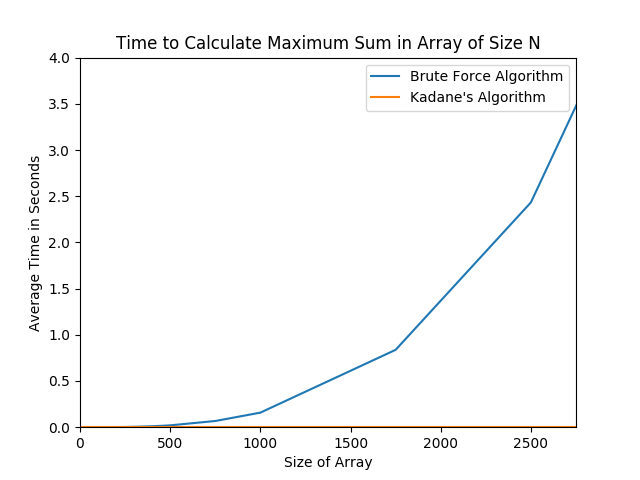
\includegraphics[width=0.75\textwidth] {python/avgTimeGraph.png}
	}
	\caption{
		\label{fig:my-label} Graph of Brute Force vs Kadane Timing
	}
	\end{figure}

	\section{Conclusions}

\end{document}
